% Options for packages loaded elsewhere
\PassOptionsToPackage{unicode}{hyperref}
\PassOptionsToPackage{hyphens}{url}
%
\documentclass[
]{article}
\usepackage{lmodern}
\usepackage{amssymb,amsmath}
\usepackage{ifxetex,ifluatex}
\ifnum 0\ifxetex 1\fi\ifluatex 1\fi=0 % if pdftex
  \usepackage[T1]{fontenc}
  \usepackage[utf8]{inputenc}
  \usepackage{textcomp} % provide euro and other symbols
\else % if luatex or xetex
  \usepackage{unicode-math}
  \defaultfontfeatures{Scale=MatchLowercase}
  \defaultfontfeatures[\rmfamily]{Ligatures=TeX,Scale=1}
\fi
% Use upquote if available, for straight quotes in verbatim environments
\IfFileExists{upquote.sty}{\usepackage{upquote}}{}
\IfFileExists{microtype.sty}{% use microtype if available
  \usepackage[]{microtype}
  \UseMicrotypeSet[protrusion]{basicmath} % disable protrusion for tt fonts
}{}
\makeatletter
\@ifundefined{KOMAClassName}{% if non-KOMA class
  \IfFileExists{parskip.sty}{%
    \usepackage{parskip}
  }{% else
    \setlength{\parindent}{0pt}
    \setlength{\parskip}{6pt plus 2pt minus 1pt}}
}{% if KOMA class
  \KOMAoptions{parskip=half}}
\makeatother
\usepackage{xcolor}
\IfFileExists{xurl.sty}{\usepackage{xurl}}{} % add URL line breaks if available
\IfFileExists{bookmark.sty}{\usepackage{bookmark}}{\usepackage{hyperref}}
\hypersetup{
  pdftitle={Project Report},
  pdfauthor={Caroline Andy, Vasili Fokaidis, Stella Li, Tessa Senders, Lily Wang},
  hidelinks,
  pdfcreator={LaTeX via pandoc}}
\urlstyle{same} % disable monospaced font for URLs
\usepackage[margin=1in]{geometry}
\usepackage{graphicx,grffile}
\makeatletter
\def\maxwidth{\ifdim\Gin@nat@width>\linewidth\linewidth\else\Gin@nat@width\fi}
\def\maxheight{\ifdim\Gin@nat@height>\textheight\textheight\else\Gin@nat@height\fi}
\makeatother
% Scale images if necessary, so that they will not overflow the page
% margins by default, and it is still possible to overwrite the defaults
% using explicit options in \includegraphics[width, height, ...]{}
\setkeys{Gin}{width=\maxwidth,height=\maxheight,keepaspectratio}
% Set default figure placement to htbp
\makeatletter
\def\fps@figure{htbp}
\makeatother
\setlength{\emergencystretch}{3em} % prevent overfull lines
\providecommand{\tightlist}{%
  \setlength{\itemsep}{0pt}\setlength{\parskip}{0pt}}
\setcounter{secnumdepth}{-\maxdimen} % remove section numbering
\usepackage{booktabs}
\usepackage{longtable}
\usepackage{array}
\usepackage{multirow}
\usepackage{wrapfig}
\usepackage{float}
\usepackage{colortbl}
\usepackage{pdflscape}
\usepackage{tabu}
\usepackage{threeparttable}
\usepackage{threeparttablex}
\usepackage[normalem]{ulem}
\usepackage{makecell}
\usepackage{xcolor}

\title{Project Report}
\author{Caroline Andy, Vasili Fokaidis, Stella Li, Tessa Senders, Lily Wang}
\date{12/11/2020}

\begin{document}
\maketitle

\hypertarget{abstract}{%
\subsection{Abstract}\label{abstract}}

\textbf{Background:}~ Hate crimes are a growing public health threat in
the United States and are the highest priority of the FBI's civil rights
program (Miller et al., 2016). Existing research suggests that various
community-level socioeconomic factors, such as income inequality, are
associated with hate crime rate.

\textbf{Objectives:}\\
We aimed to analyze the association between state-level variables and
rate of population-adjusted hate incidents using data reported to the
Southern Poverty Law Center and analyzed in a 2017 FiveThrityEight
article (Majumder, 2017).

\textbf{Methods:}\\
The data used for this project included state-level hate crime rates per
100,000 individuals in the population, as reported by the Southern
Poverty Law Center in 2016. Data elements also included socioeconomic
factors that are hypothesized to be associated with hate crime.

The association between these socioeconomic factors and the hate crime
rate outcome were examined using multivariable linear regression
analysis. We then used automated and criterion-based approaches,
considering the body of scientific evidence with regard to significant
and practically important factors associated with hate crimes, to
identify a regression model which optimizes parsimony and goodness of
fit.

Multicollinearity of covariates, outliers, and variable interaction were
also tested for and considered in model development. Model goodness of
fit and predictive performance were assessed through model diagnostics
and validation. All abovementioned steps were performed before and after
removing any outliers in the data.

\textbf{Results and Conclusions:}\\
Gini Index (an indicator of wealth inequality) and percent population
with a high school degree were both significant predictors of
state-level hate crime rate when controlling for all other covariates.
When these two predictors were the only parameters included in the model
they were both positively associated with the outcome.

Multicollinearity tests showed possible correlation between median
household income and percentage of population with a high school degree,
as well as the percent non-citizen and percent non-white variables. No
statistically significant interactions were identified between any
variables in regression modeling.

Our identified model optimizing goodness of fit and predictive
performance contained only the Gini Index and percent population with a
high school degree as parameters, both of which were significant.
Washington DC, the single outlier in the data, was found to be an
influential point, as its absence from the data nullified the
significance of the Gini Index predictor in the two-parameter model.

\hypertarget{introduction}{%
\subsection{Introduction}\label{introduction}}

As of 2020, the national rate of hate crimes in the United States is at
its highest level in over a decade {[}``FBI Incidents and Offenses,''
2019{]}. In the days following the 2016 US Presidential election, an
average of 90 hate crimes per day were reported to the Southern Poverty
Law Center (Miller et al., 2016).

Existing research suggests that community-level socioeconomic factors
such as racial breakdown, population density, level of educational
attainment, and economic considerations (median income, poverty level,
job availability) may be significant predictors of regional and
state-level rates of hate crimes (``FBI: Variables Affecting Crime,''
2012, Shively, 2005, Van Dyke et al., 2014). A 2017 FiveThirtyEight
article titled, ``Higher Rates Of Hate Crimes Are Tied To Income
Inequality,'' used 2016 FBI and Southern Poverty Law Center data to
assess the association between state-level hate crime rate and select
socioeconomic variables (Majumder, 2017).

For this project, we used this dataset to critically analyze this
research team's findings to identify state-level variables associated
with rates of hate crimes, and to generate a high performing predictive
model for population-adjusted hate incidents in the United States.

\hypertarget{methods}{%
\subsection{Methods}\label{methods}}

\hypertarget{data-exploration}{%
\paragraph{Data Exploration}\label{data-exploration}}

The data used for this project included state-level hate crime rates
(hate crimes per 100,000 population), as reported by the Southern
Poverty Law Center during the first weeks of November, 2016. Collected
state-level demographic variables include:

\begin{itemize}
\tightlist
\item
  Unemployment rate (high vs low) (as of 2016)
\item
  Urbanization (high vs low) (as of 2015)
\item
  Median household income (as of 2016)
\item
  Percent of residents with a high school degree (as of 2009)
\item
  Percent of residents who are non-citizens (as of 2015)
\item
  Income Gini coefficient (a measure of the extent to which the
  distribution of income among individuals within an economy deviates
  from a perfectly equal distribution; as of 2015)
\item
  Percent of residents who are non-White (as of 2015)
\end{itemize}

First, we investigated the extent of missing data in our dataset. Four
states -- Hawaii, North Dakota, South Dakota, and Wyoming -- did not
report hate crime rate data, and thus were excluded from subsequent
analyses. Three states -- Maine, Mississippi, and South Dakota -- did
not report their percent of residents who were non-citizens. The
District of Columbia (DC) was included as a state for the purposes of
these analyses.

We then generated a table of descriptive statistics, including the mean,
median, range (min-max), interquartile range, and count of missing
entries for each numeric variable, and category percent breakdowns and
count of missing entries for categorical variables (Table 1).

Using these data, our goal was to assess which of the collected
variables, if any, are statistically significantly associated (at a 0.05
significance level) with population-adjusted hate incidents in the
United States. To do so, we employed multivariable linear regression
modeling, which operates under several assumptions, which include
residual homoscedasticity (constant variance) and normality. To test
whether these assumption were met, we first generated an overlaid
density and histogram plot of population-adjusted hate incidents per
100,000 population, which showed a strong departure from standard normal
distribution and significant right skewness. Thus, we performed a Box
Cox transformation to isolate the `best' power transformation on the
hate crimes rate variable to achieve normal residuals.

To identify any outliers, and thus potential influential points, we
plotted the hate crime rate by state (Figure 3). We then generated
residuals vs fitted, normal Q-Q, scale-location, and residuals vs
leverage plots for a linear regression model that regressed the
transformed hate crime rate onto all possible covariates (Figure 4).
Specifically, we used the Residuals vs Leverage plot to identify
outliers. Points outside of Cook's Distance on the Residuals vs Leverage
plot were considered potential influential points.

Any states that were deemed to be outliers were included in the
subsequent analyses, but the same analyses were also run a second time
on the dataset excluding the outliers for comparison in order to
determine if the outlier was indeed influencing the results of our
analyses.

\hypertarget{multicollinearity-and-interactions}{%
\paragraph{Multicollinearity and
Interactions}\label{multicollinearity-and-interactions}}

To investigate the existence of multicollinearity between each of the
continuous variables, we generated a correlation matrix. We decided that
any correlation coefficient of 0.6 and above may suggest
multicollinearity; thus, in these instances, at least one of those
correlated variables were dropped during subsequent model development.
Additionally, we calculated the variance inflation factors (VIFs) for
all variables, which quantify the degree of multicollinearity between
the given predictor all other remaining covariates.

Next, we plotted potential interactions between the continuous variables
and each categorical variable, urbanization and unemployment, to see if
the effect of each continuous variable on the log rate of hate crimes is
different with respect to the levels of either urbanization or
unemployment. These plots were created once including outliers and once
excluding outliers. We then formally tested for significant interactions
between any variable pairs with intersecting lines. All interaction
tests were performed on datasets containing and not containing any
observed outliers.

\hypertarget{model-development-and-validation}{%
\paragraph{Model Development and
Validation}\label{model-development-and-validation}}

We began by performing two automated procedures for model variable
selection (forward and backward stepwise selection). We then used two
criterion based approaches (Mallow's Cp and adjusted r-squared). These
two criterion based approaches each generated the best performing model
which optimizes the given criterion for each possible number of
predictors. The first of these approaches used Mallow's Cp criterion,
which compares the predictive ability of model subsets to the full
model. The most ideal model will have a Cp value less than or equal to
the number of predictors in the model. To visualize these results, we
generated a plot containing the Cp criterion distribution for the top
performing model for each number of predictors (Figure 8).

The next approach used adjusted r-squared which favors models with a
smaller sum of squares error (the sum of the differences between each
observed value and predicted value) but also penalizes for additional
predictors. By this criterion, the best model will have the highest
adjusted r-squared value. We generated a plot of the distribution of the
adjusted R squared statistic for the top performing model for each
number of included predictors (Figure 9).

Using these results, we then identified the two best models which
maximize parsimony, interpretability and practical application, which
takes into account variables deemed to be significant and practically
important in existing literature. We then compared these two models
using an analysis of variance (a partial F-test for nested models).

We ensured that the model selected after this test did not violate any
of the assumptions of linear regression by considering four main
diagnostic plots: residuals vs fitted, normal Q-Q, scale-location, and
residuals vs leverage.

We repeated this process of model selection on the dataset excluding any
observed outliers.

To assess the predictive performance of the top two identified models,
we performed 5-fold Cross Validation (CV) on each including and
excluding outliers. We evaluated the model performance based on their
root mean square errors (RMSE) and adjusted r-squared values generated
from CV. A lower RMSE is desirable as it indicates a larger proportion
of variance explained by the model. We also compared the values
generated from CV to the values from the original regression model to
ensure the model performs well on new data.

\hypertarget{results}{%
\subsection{Results}\label{results}}

\hypertarget{data-exploration-1}{%
\paragraph{Data Exploration}\label{data-exploration-1}}

The generated Box Cox transformation plot indicates that a lambda of 0
(i.e.~a natural logarithmic transformation of the hate crimes rate
outcome) would most closely approximate normal distribution (Figure 2).
Thus, we operated moving forward in model development using the natural
log of hate crimes rate as the outcome of interest.

Examining the Residuals vs Leverage plot generated from the regression
model including all possible covariates, we see that District of
Columbia is clearly outside of the Cook's Distance line; thus we
concluded that this point is an outlier and a potential influential
point (Figure \#).

A table of basic descriptive statistics for the collected socioeconomic
variables is included in the appendix (Table 1). Notably, the hate crime
rate per 100,000 individuals had a mean of 0.315 and range of 0.067 to
1.522, indicating considerable variation in state-level hate crime rates
per 100,000 individuals. The Gini Index values, ranging from 0.419 to
0.532 across the included states, indicating substantial state-level
income inequality in the overall dataset. A majority of states had both
high urbanization and unemployment (51.1\% each) (Table 1).

\hypertarget{multicollinearity-and-interactions-1}{%
\paragraph{Multicollinearity and
Interactions}\label{multicollinearity-and-interactions-1}}

Of the continuous variables, percent non-citizen and percent non-white
have a correlation coefficient of 0.753, and median household income and
percentage of population with a high school degree have a correlation
coefficient of 0.651, both of which may suggest multicollinearity. All
other correlation coefficients do not suggest multi-collinearity (Table
2).

Use of variance inflation factors (VIFs) showed that the percent
population without a high school degree (3.895), percent non-citizen
(3.728), percent non-white (3.236) and median household income (3.108)
have the highest degrees of multicollinearity between all other
predictors. These values approach but do not exceed 4, the generally
accepted value which denotes the need for further investigation and/or
consideration of multicollinearity corrections.

For the dataset containing DC, the interaction plots suggest potential
interaction between unemployment and median household income, as well as
between unemployment and percent population of high school graduates, as
seen by the differing directions in slope (crossing lines). The
urbanization interaction plots for these data suggest that there may be
potential interaction between urbanization and each of the following
variables: Gini Index, median household income, percent non-citizen, and
percent population of high school graduates.

For the dataset excluding DC, the interaction plots show potential
interaction between unemployment and Gini Index as well as between
unemployment and percent population of high school graduates. The
urbanization interaction plots for these data suggest potential
interaction between urbanization and median household income as well as
between urbanization and percent population of high school graduates.

When performing regression analyses for all of the above interactions
for each dataset, no interactions were found to be statistically
significant at a 0.05 significance level.

\hypertarget{model-development-and-validation-1}{%
\paragraph{Model Development and
Validation}\label{model-development-and-validation-1}}

We began our regression analyses by running linear regression models
containing all possible predictors for both the untransformed hate crime
rate and the natural log transformed hate crime rate. Our results
support the conclusions drawn in the FiveThirtyEight article: that the
Gini Index was the most significant independent predictor of state hate
crime rate when controlling for all other covariates and that the
percent high school graduates variable was the only other statistically
and independently significant variable (Majumder, 2017).

The model proposed during forward stepwise selection contained all
variables provided in the original dataset (Adjusted R-squared =
0.1849). The model generated through backward stepwise selection was
much more parsimonious and had a substantially higher adjusted R squared
(Adjusted R-squared = 0.2868). The only included predictors were the
Gini Index, and the percent of high school graduates, both of which were
significant. When DC is removed from the dataset, however, the Gini
Index is no longer statistically significant at a 0.05 significance
level, indicating that DC is an influential point. The adjusted
R-squared of the two-predictor model decreases as well when DC is
removed (from 0.2541 to 0.1185).

Both Mallow's Cp and the adjusted r-squared criterion confirmed that the
best model that includes two variables contains Gini Index and the
percent of high school graduates. Further, the plot for Mallow's Cp
showed that the model with only two predictors had the lowest Cp value
as compared to the best performing model of all other possible numbers
of predictors. The plot for the adjusted r-squared criterion showed that
the model with 3 predictors (Gini Index, the percent of high school
graduates, and unemployment) had the highest adjusted r-squared value.
However, the adjusted r-squared for this model was less than 6\% greater
than the adjusted r-squared for the model with only 2 covariates,
suggesting that their performance is not significantly different with
regard to this criterion. Further the partial F-test for nested models
shows that adding the unemployment variable does not significantly
improve the model. All of these results hold true when DC is removed
from the dataset.

Looking at the diagnostic plots for the two-covariate model that
includes DC shows no obvious violation of the assumptions. The points in
the Residuals vs Fitted plot seem randomly scattered around the line at
0 indicating the assumption of homoscedasticity is met. The points
follow a straight line in the Q-Q plot indicating the assumption of
normality is met. The Residuals vs Leverage plot however indicates that
point 9 (DC) may be an outlier. When DC is removed all the diagnostic
plots remain similar except that there is no longer any outliers
indicated by the Residuals vs Leverage plot.

The association between the two variables and the natural log of hate
crime rates is positive whether DC is included in the data or not. For a
one unit increase in the gini index, there is a 16.486 expected increase
in the natural log of hate crime rates holding the percent of HS
graduates constant (when excluding DC the expected increase is 10.811).
For a one unit increase in the percent of HS graduates, there is a
11.554 expected increase in the natural log of hate crime rates holding
the gini index constant (when excluding DC the expected increase is
9.509).

Through cross-validation, we determined that the aforementioned
two-predictor model also had better predictive performance than the
three-predictor model when including DC. The CV root mean squared error
(RMSE) values are essentially equivalent (0.5948853 for 2 covariates vs
0.6038494 for 3 covariates) and the CV adjusted r-squared is slightly
higher for the two-predictor model (0.2943289 vs 0.2783783). When
excluding DC, the two different models have virtually the same
predictive performance. Both have similar CV RMSE values and the CV
adjusted r-squared for the three-predictor model is only slightly higher
than the two-predictor model (0.1730294 vs 0.1530310). This indicates
that the addition of unemployment as a third predictor did not
significantly add to model performance whether DC is included or not
(Table 3). The two-predictor model, whether DC is included or not,
performs well as a predictive model since the model's RMSE and adjusted
r-squared are very similar to the CV average RMSE and adjusted
r-squared.

{[}ADD FIGURE NUMBER AND THEN CITE SOMEWHERE ABOVE{]}

\hypertarget{discussionconclusion}{%
\subsection{Discussion/Conclusion}\label{discussionconclusion}}

After extensive analyses and modeling, we found that the optimal model
in terms of goodness of fit and predictive value contained the Gini
Index and percent population with a high school degree, with the latter
variable being a more significant predictor of hate crime in this
two-parameter model. However, these two predictors only accounted for
25.4\% of the variability in the data. This implies other variables not
in the data should be included in future studies of hate crime rates.
Such variables may include variables related to the politics of people
in the state or the percent of the population that are LGBTQ+ or percent
of the population that belongs to a religious minority as one study
showed that religious hate crimes are on the rise (``Incidents and
Offenses.'' FBI, FBI, 29 Oct.~2019).

The change in predictor significance of Gini Index and the adjusted
r-squared between the model including and excluding DC suggests it is
indeed an influential point. DC has the highest hate crime rate and the
highest income inequality out of all the states.

ADD PARAGRAPH-WHY IS THIS STUDY IMPORTANT???

Unfortunately the data for hate crime rates was missing for four states.
These four states may have drastically different hate crime rates than
the rest of the states and could potentially change the significance of
the predictors and impact the predictive ability of our models,
therefore the results of this study may not be generalizable to the
entire US. Another limitation of our analyses is that we only tested for
interactions between the two ctageorical variables and each of the
continuous variables because these interactions are easier to understand
and stratify the data by. However, there could be interactions between
the continuous variables and even three-way interactions that explain
more of the variability in the data.

It is important to note that a natural logarithmic transformation of the
outcome was performed in order to satisfy the assumptions of linear
regression (residual homoscedasticity and normality) which impacts the
modeling results.

-why is this important? - limitations -assumptions - suggestions for
possible future studies

``Each figure and table should be of publishable quality and well
notated, i.e., labeled and/or captioned''

\hypertarget{figures-and-tables}{%
\subsection{Figures and Tables}\label{figures-and-tables}}

\begin{table}

\caption{\label{tab:unnamed-chunk-2}Descriptive Statistics of States Reporting Hate Crimes}
\centering
\begin{tabular}[t]{l|l}
\hline
 & Overall (N=47)\\
\hline
**Unemployment** & \\
\hline
\&nbsp;\&nbsp;\&nbsp;high & 24 (51.1\%)\\
\hline
\&nbsp;\&nbsp;\&nbsp;low & 23 (48.9\%)\\
\hline
\&nbsp;\&nbsp;\&nbsp;Missing & 0\\
\hline
**Urbanization** & \\
\hline
\&nbsp;\&nbsp;\&nbsp;low & 23 (48.9\%)\\
\hline
\&nbsp;\&nbsp;\&nbsp;high & 24 (51.1\%)\\
\hline
\&nbsp;\&nbsp;\&nbsp;Missing & 0\\
\hline
**Median Household Income** & \\
\hline
\&nbsp;\&nbsp;\&nbsp;Mean (SD) & 54802.298 (9255.117)\\
\hline
\&nbsp;\&nbsp;\&nbsp;Median (Q1, Q3) & 54310.000 (47629.500, 60597.500)\\
\hline
\&nbsp;\&nbsp;\&nbsp;Min - Max & 35521.000 - 76165.000\\
\hline
\&nbsp;\&nbsp;\&nbsp;Missing & 0\\
\hline
**\% Adults >25yrs With HS Degree** & \\
\hline
\&nbsp;\&nbsp;\&nbsp;Mean (SD) & 0.866 (0.034)\\
\hline
\&nbsp;\&nbsp;\&nbsp;Median (Q1, Q3) & 0.871 (0.839, 0.895)\\
\hline
\&nbsp;\&nbsp;\&nbsp;Min - Max & 0.799 - 0.915\\
\hline
\&nbsp;\&nbsp;\&nbsp;Missing & 0\\
\hline
**\% of Population Not U.S. Citizens** & \\
\hline
\&nbsp;\&nbsp;\&nbsp;Mean (SD) & 0.055 (0.031)\\
\hline
\&nbsp;\&nbsp;\&nbsp;Median (Q1, Q3) & 0.050 (0.030, 0.080)\\
\hline
\&nbsp;\&nbsp;\&nbsp;Min - Max & 0.010 - 0.130\\
\hline
\&nbsp;\&nbsp;\&nbsp;Missing & 2\\
\hline
**Gini Index** & \\
\hline
\&nbsp;\&nbsp;\&nbsp;Mean (SD) & 0.456 (0.021)\\
\hline
\&nbsp;\&nbsp;\&nbsp;Median (Q1, Q3) & 0.455 (0.441, 0.468)\\
\hline
\&nbsp;\&nbsp;\&nbsp;Min - Max & 0.419 - 0.532\\
\hline
\&nbsp;\&nbsp;\&nbsp;Missing & 0\\
\hline
**\% of Population Not White** & \\
\hline
\&nbsp;\&nbsp;\&nbsp;Mean (SD) & 0.315 (0.150)\\
\hline
\&nbsp;\&nbsp;\&nbsp;Median (Q1, Q3) & 0.300 (0.205, 0.420)\\
\hline
\&nbsp;\&nbsp;\&nbsp;Min - Max & 0.060 - 0.630\\
\hline
\&nbsp;\&nbsp;\&nbsp;Missing & 0\\
\hline
**Hate Crime Rate Per 100k** & \\
\hline
\&nbsp;\&nbsp;\&nbsp;Mean (SD) & 0.304 (0.253)\\
\hline
\&nbsp;\&nbsp;\&nbsp;Median (Q1, Q3) & 0.226 (0.143, 0.357)\\
\hline
\&nbsp;\&nbsp;\&nbsp;Min - Max & 0.067 - 1.522\\
\hline
\&nbsp;\&nbsp;\&nbsp;Missing & 0\\
\hline
\multicolumn{2}{l}{\rule{0pt}{1em}\textit{Note: }}\\
\multicolumn{2}{l}{\rule{0pt}{1em}This table shows the adjusted R\textasciicircum{}2 and RMSE values for two models with DC and two models without DC for two and three predictors in each type of model.}\\
\end{tabular}
\end{table}

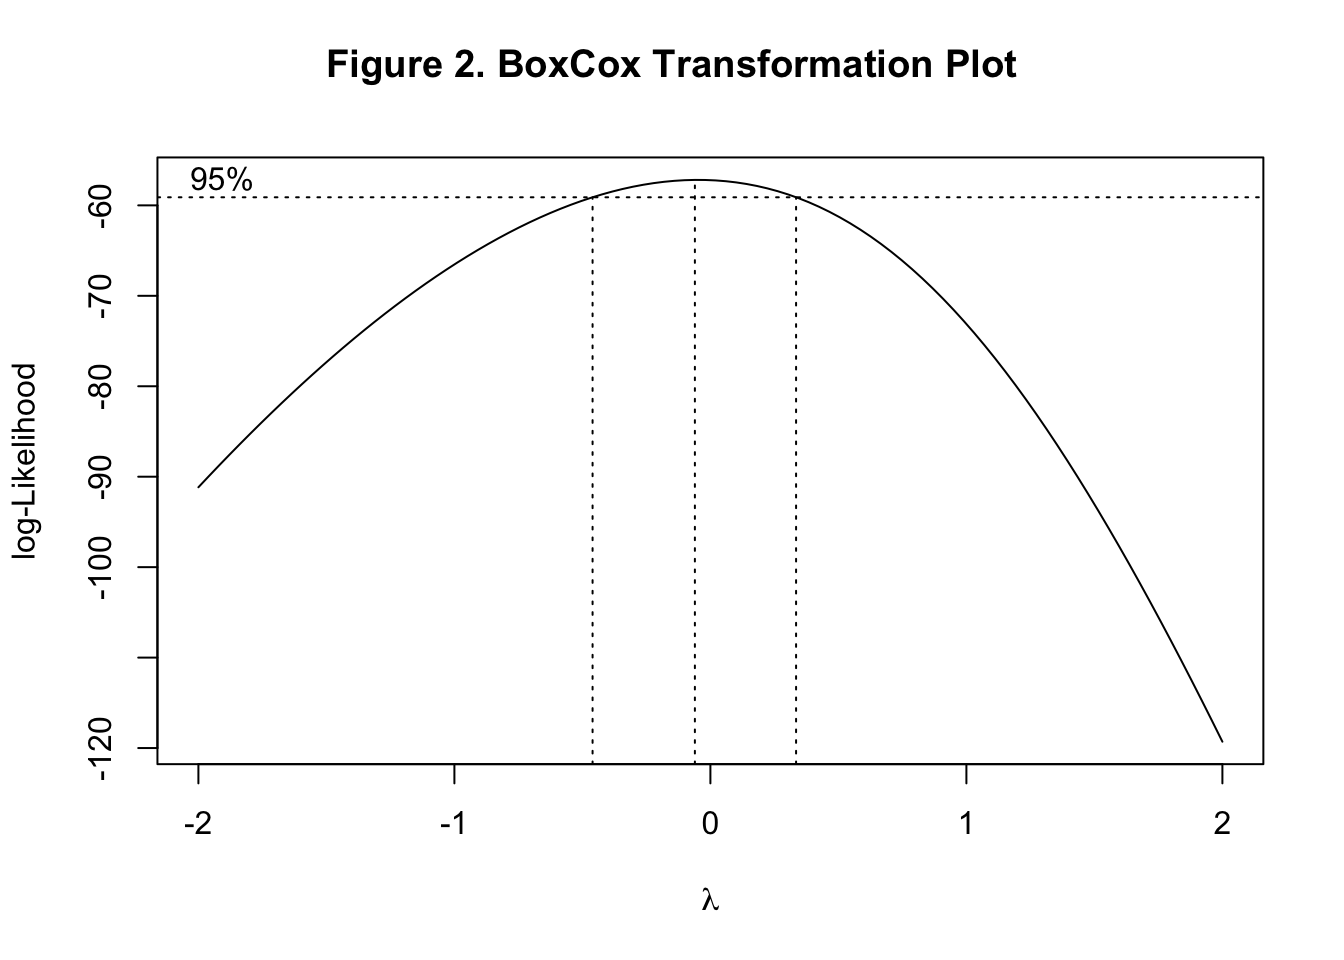
\includegraphics{project_report_files/figure-latex/unnamed-chunk-3-1.pdf}

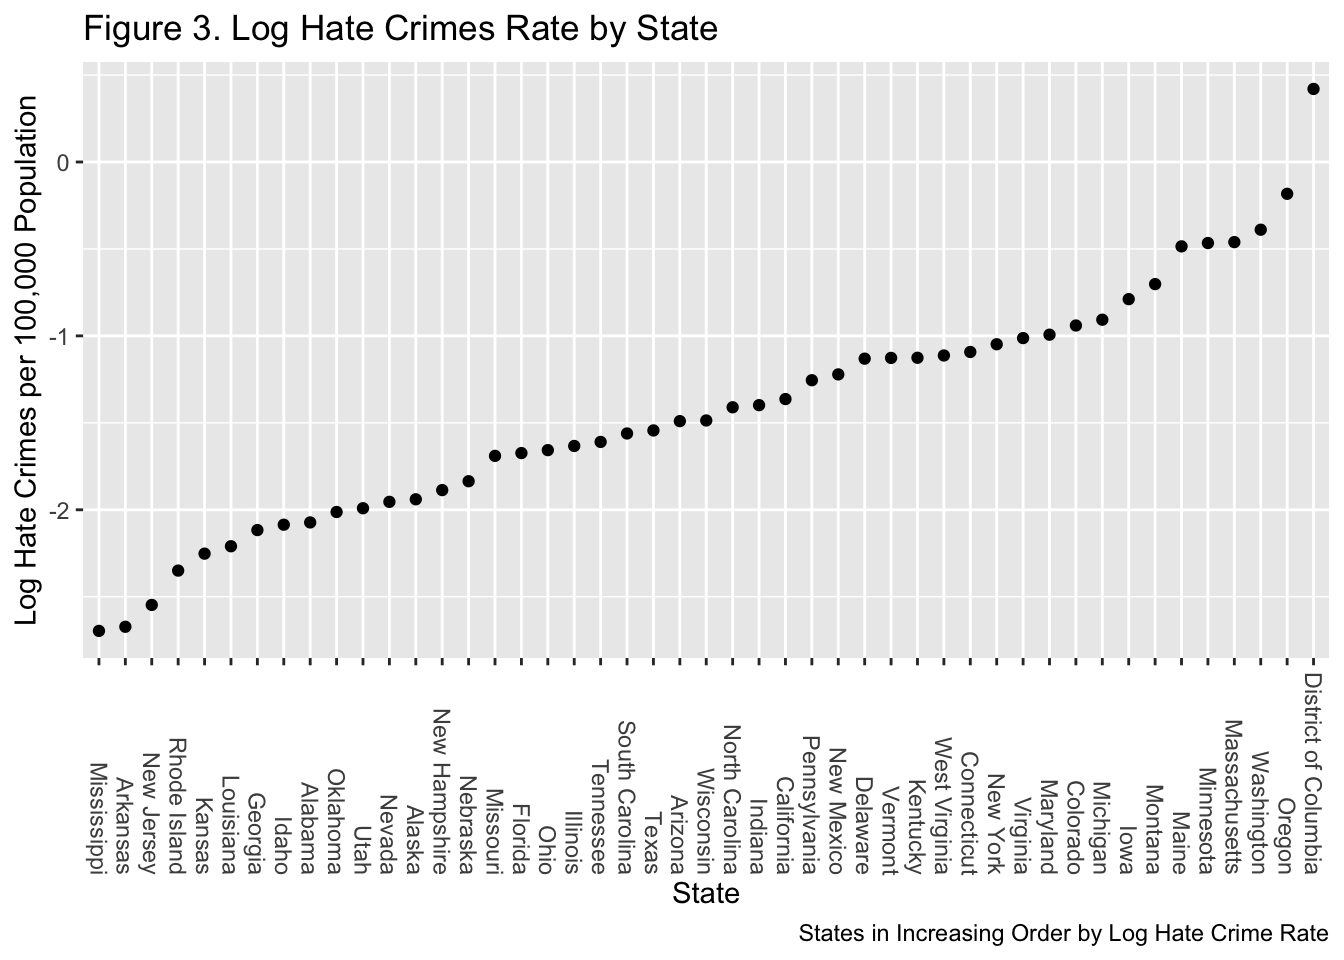
\includegraphics{project_report_files/figure-latex/unnamed-chunk-4-1.pdf}

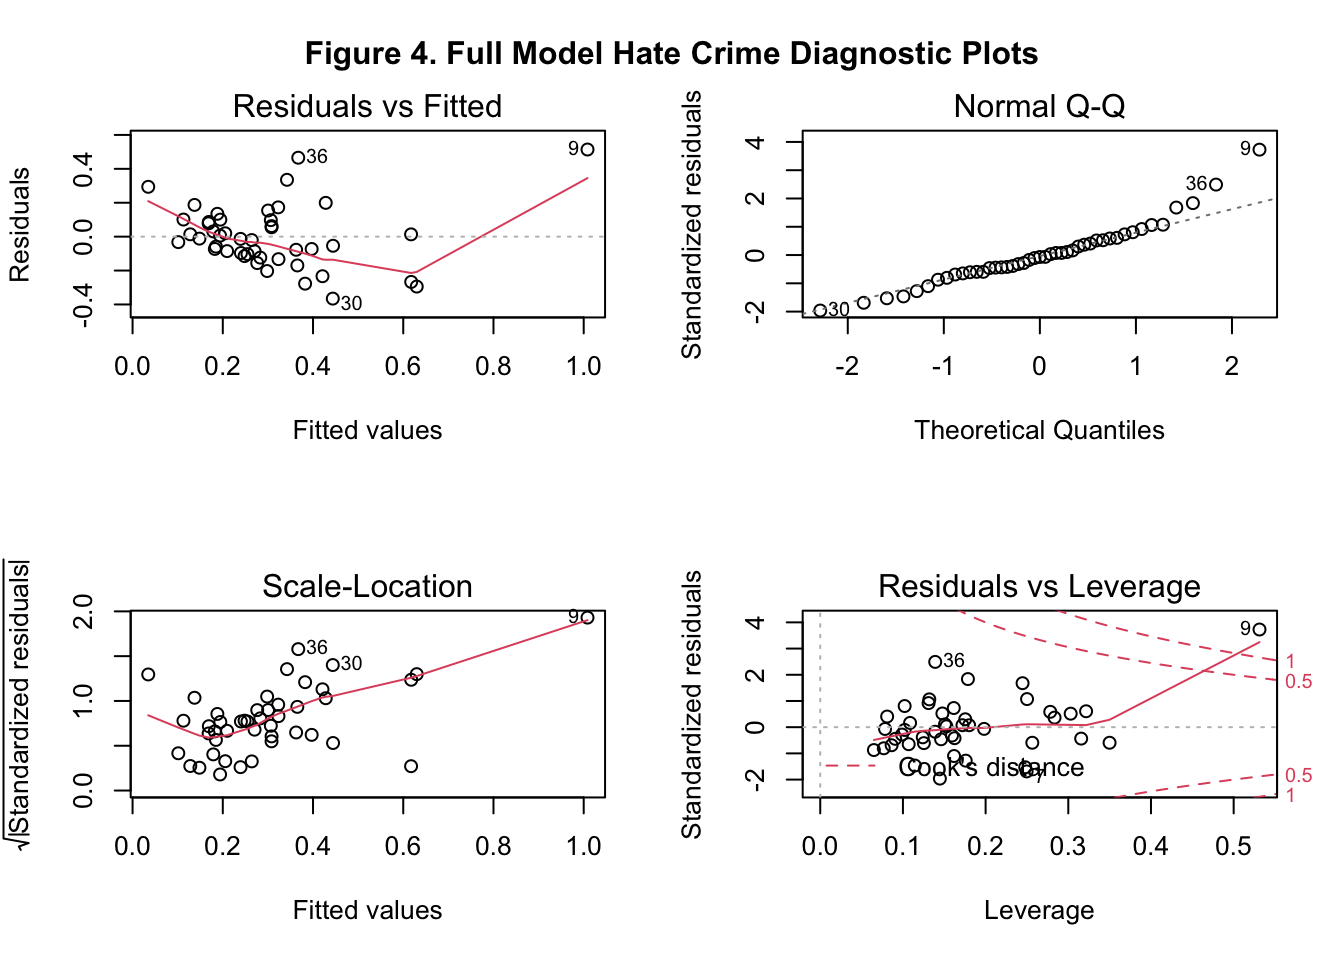
\includegraphics{project_report_files/figure-latex/unnamed-chunk-5-1.pdf}

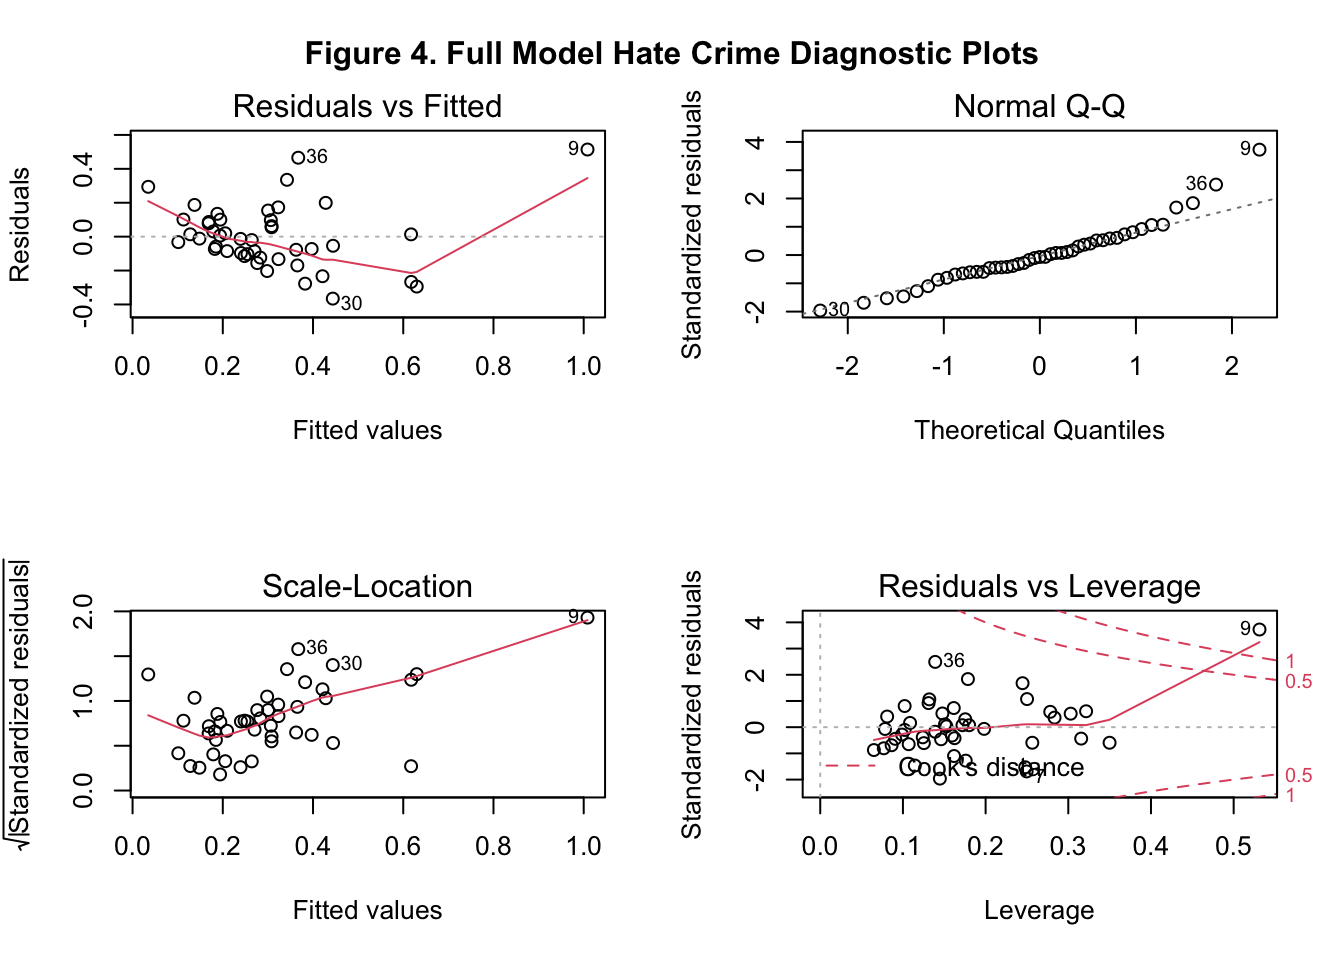
\includegraphics{project_report_files/figure-latex/unnamed-chunk-6-1.pdf}
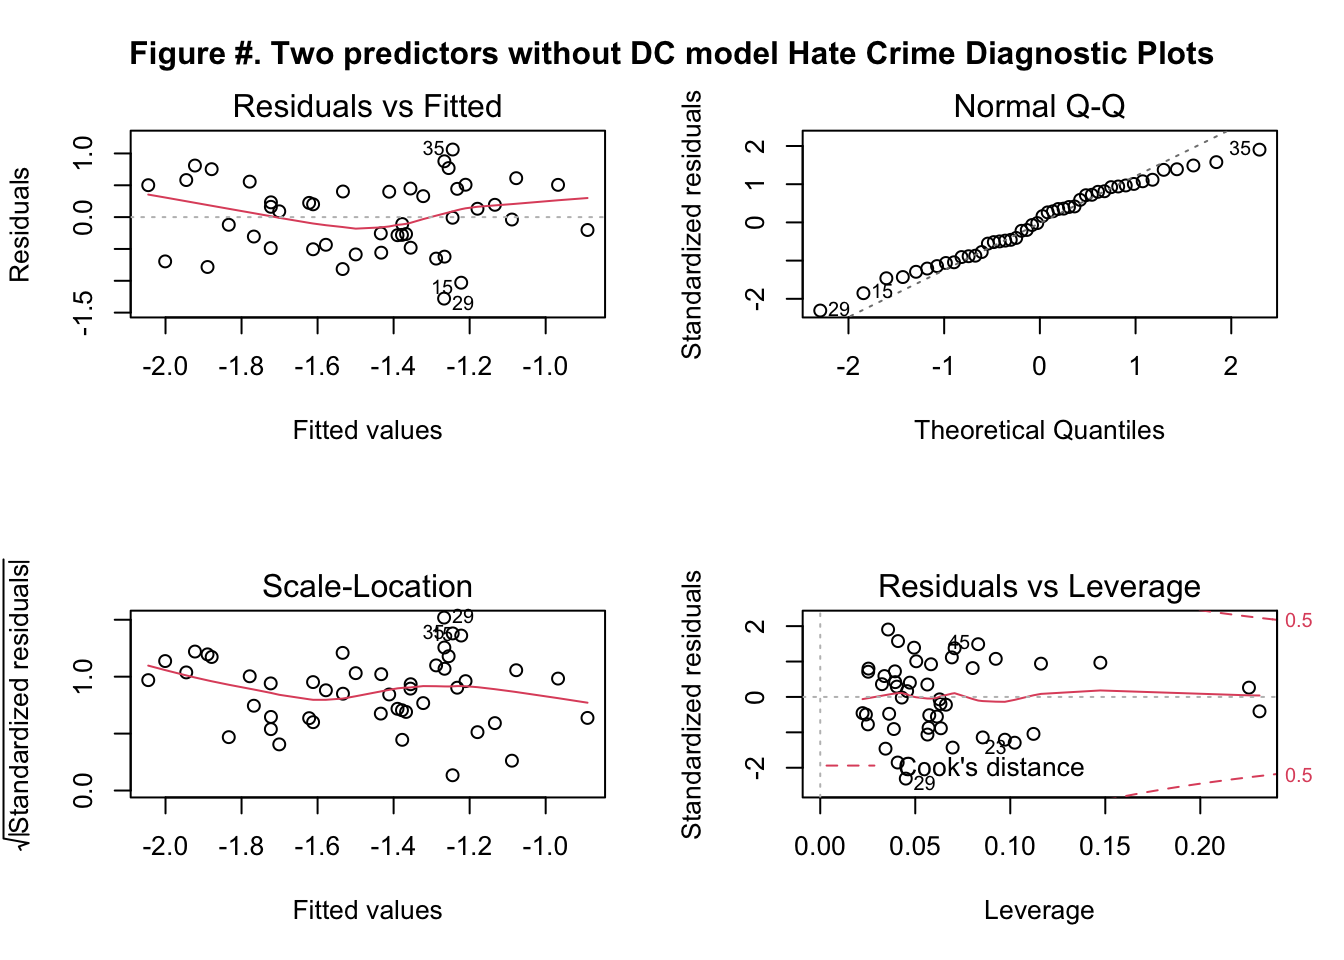
\includegraphics{project_report_files/figure-latex/unnamed-chunk-6-2.pdf}

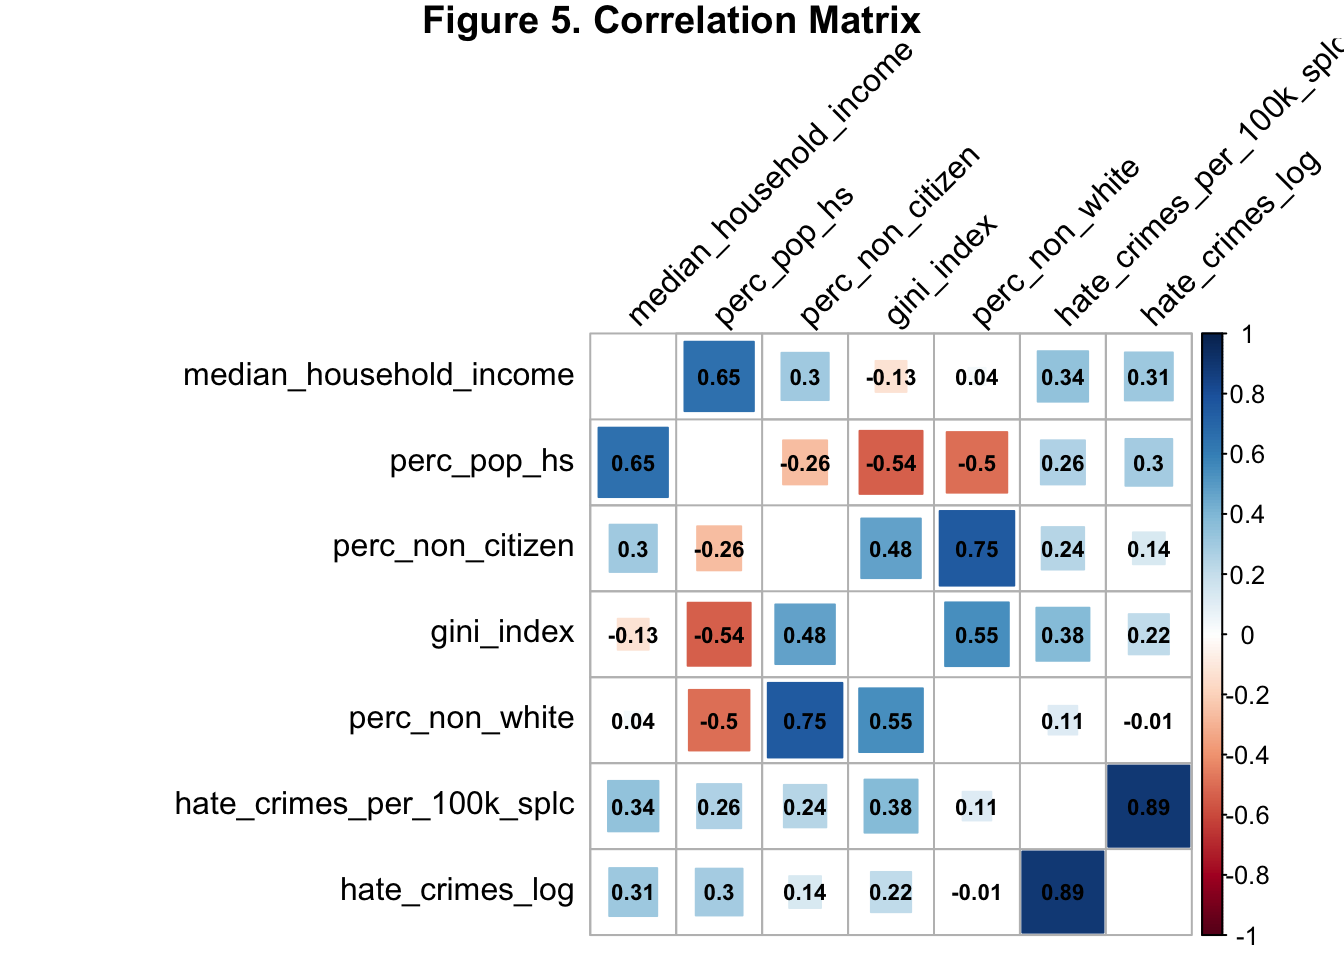
\includegraphics{project_report_files/figure-latex/unnamed-chunk-7-1.pdf}

\begin{table}

\caption{\label{tab:unnamed-chunk-8}Table of variance inflation factors for each variable.}
\centering
\begin{tabular}[t]{l|r}
\hline
  & VIF\\
\hline
`Unemployment ` & 1.426\\
\hline
`Urbanization ` & 1.983\\
\hline
`Median Household Income` & 3.108\\
\hline
`\% Adults >25yrs With HS Degree` & 3.895\\
\hline
`\% of Population Not U.S. Citizens` & 3.728\\
\hline
`Gini Index` & 1.845\\
\hline
`\% of Population Not White` & 3.236\\
\hline
\end{tabular}
\end{table}

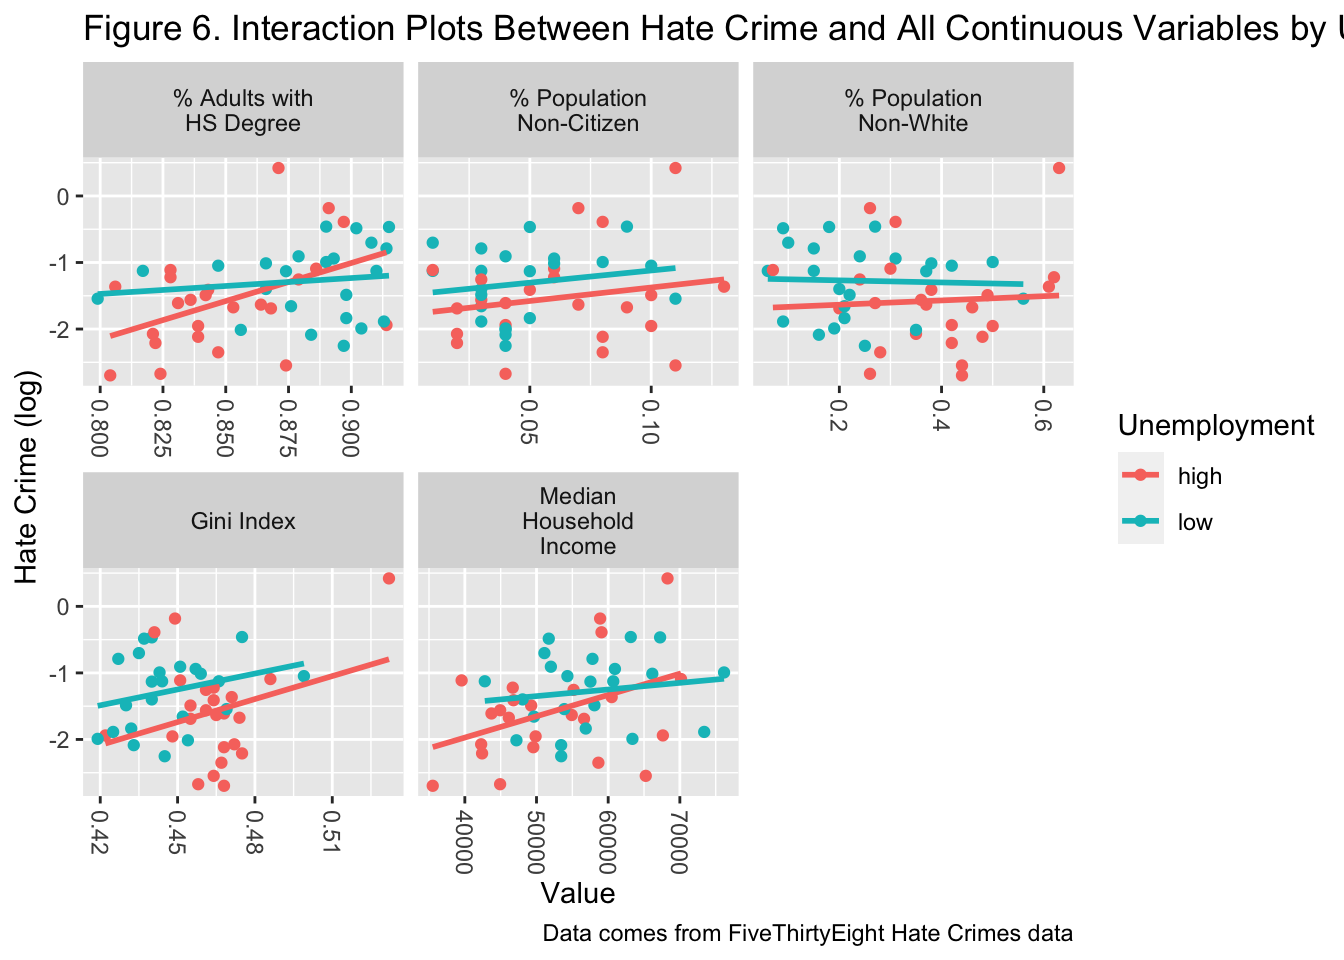
\includegraphics{project_report_files/figure-latex/unnamed-chunk-9-1.pdf}

\includegraphics{project_report_files/figure-latex/unnamed-chunk-10-1.pdf}

\includegraphics{project_report_files/figure-latex/unnamed-chunk-11-1.pdf}

\begin{table}

\caption{\label{tab:unnamed-chunk-12}Comparison of Adjusted R^2 and RMSE for All Models}
\centering
\begin{tabular}[t]{l|r|r|r|r}
\hline
  & Model adjusted R\textasciicircum{}2 & Model RMSE & CV adjusted R\textasciicircum{}2 & CV RMSE\\
\hline
Two predictors with DC & 0.2541 & 0.5417445 & 0.2943289 & 0.5948853\\
\hline
Three predictors with DC & 0.2571 & 0.5341956 & 0.2783783 & 0.6038494\\
\hline
Two predictors without DC & 0.1185 & 0.5367246 & 0.1530310 & 0.5554347\\
\hline
Three predictors without DC & 0.1250 & 0.5281813 & 0.1730294 & 0.5600140\\
\hline
\end{tabular}
\end{table}

\hypertarget{references}{%
\subsection{References}\label{references}}

\begin{itemize}
\tightlist
\item
  ``Incidents and Offenses.'' FBI, FBI, 29 Oct.~2019,
  ucr.fbi.gov/hate-crime/2019/topic-pages/incidents-and-offenses.
\item
  Majumder, M. ``Higher Rates Of Hate Crimes Are Tied To Income
  Inequality.'' FiveThirtyEight, FiveThirtyEight, 23 Jan.~2017,
  fivethirtyeight.com/features/higher-rates-of-hate-crimes-are-tied-to-income-inequality/.
\item
  Miller, C., Werner-Winslow, A. ``Ten Days After: Harassment and
  Intimidation in the Aftermath of the Election.'' Southern Poverty Law
  Center, 29 Nov.~2016,
  www.splcenter.org/20161129/ten-days-after-harassment-and-intimidation-aftermath-election.\\
\item
  Shively, Michael. Abt Associates Inc, 2005, Study of Literature and
  Legislation on Hate Crime in America.
\item
  Van Dyke, N., and Tester, G. ``Dangerous Climates.'' Journal of
  Contemporary Criminal Justice, vol.~30, no. 3, 2014, pp.~290--309.,
  \url{doi:10.1177/1043986214536666}.
\item
  ``Variables Affecting Crime.'' FBI, FBI, 5 Nov.~2012,
  ucr.fbi.gov/hate-crime/2011/resources/variables-affecting-crime.
\end{itemize}

\end{document}
